
\section{Template}

\begin{frame}
  \frametitle{Acceleration Modification in the Y-axis}
  \begin{figure}
    \centering
    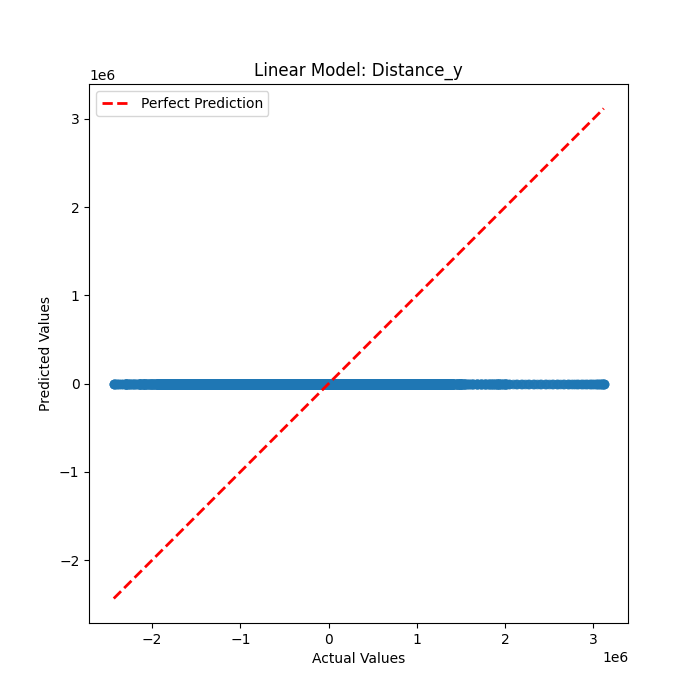
\includegraphics[width=0.5 \textwidth]{figures/acceleration_mod/acceleration_mod_dist_y.png}
  \end{figure}
\end{frame}


\begin{frame}
  \frametitle{Acceleration Modification in the Y-axis}
  \begin{figure}
    \centering
    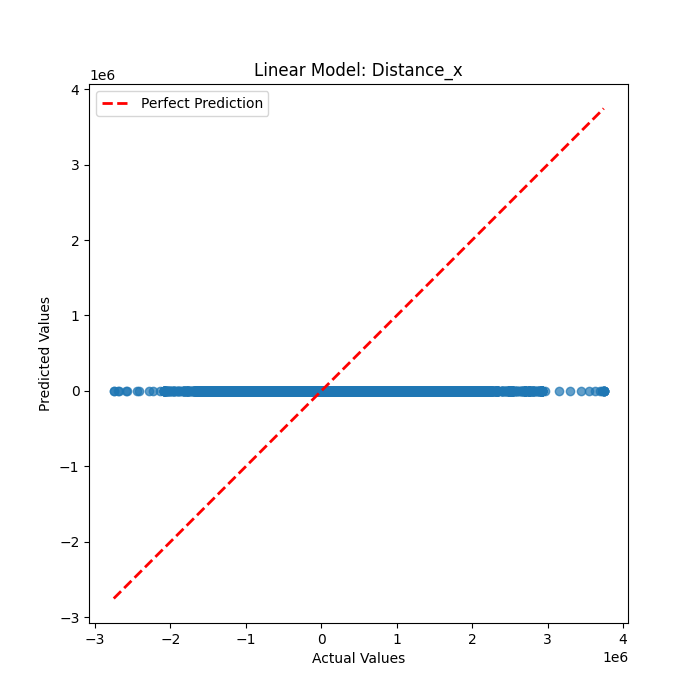
\includegraphics[width=0.5 \textwidth]{figures/acceleration_mod/acceleration_mod_dist_x.png}
  \end{figure}
\end{frame}


\begin{frame}
  \frametitle{Acceleration Modification in the Y-axis}
  \begin{figure}
    \centering
    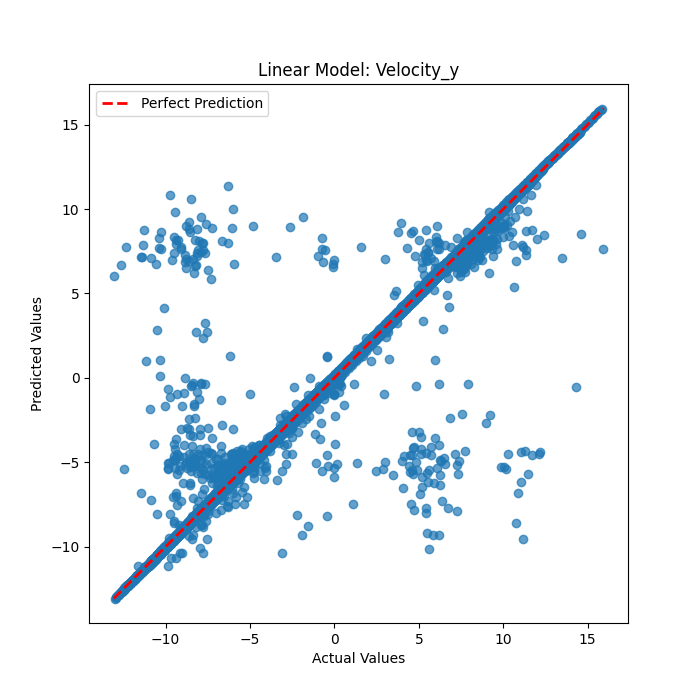
\includegraphics[width=0.5 \textwidth]{figures/acceleration_mod/acceleration_mod_vel_y.png}
  \end{figure}
\end{frame}


\begin{frame}
  \frametitle{Acceleration Modification in the Y-axis}
  \begin{figure}
    \centering
    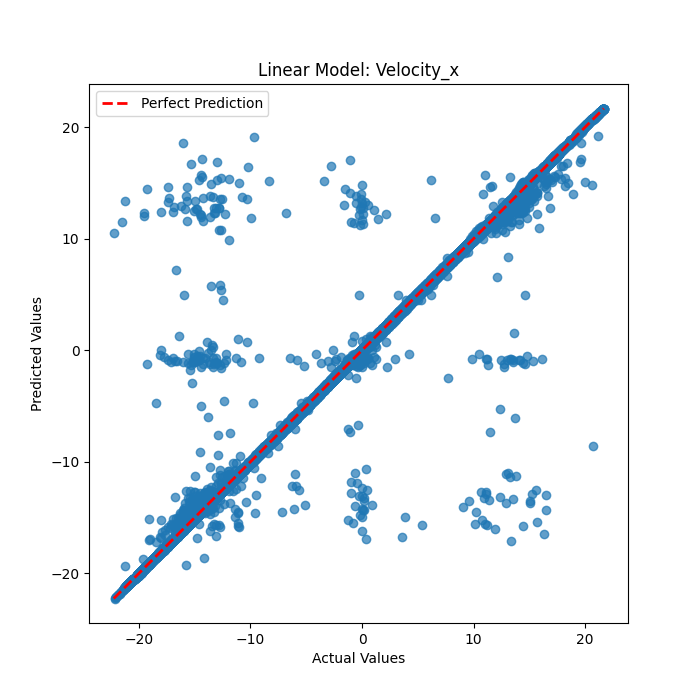
\includegraphics[width=0.5 \textwidth]{figures/acceleration_mod/acceleration_mod_vel_x.png}
  \end{figure}
\end{frame}




\begin{frame}{Motivation for Set-Based Prediction $[$1$]$}
\blfootnote{\tiny $[$1$]$ M. Althoff and S. Magdici, ``Set-based prediction of traffic participants on arbitrary road networks,'' IEEE Transactions on Intelligent Vehicles, vol. 1, no. 2, pp. 187--202, 2016.}

	\centering	
	\footnotesize
      \psfrag{o}[c][c]{obstacle}						
      \psfrag{c}[c][c]{traffic participant}
      \psfrag{e}[c][c]{ego vehicle}
      \psfrag{f}[c][c]{intended trajectory}      
      \psfrag{w}[r][c]{$t \in [t_0, t_1]$:}
      \psfrag{x}[r][c]{$t \in [t_1, t_2]$:}
      \psfrag{y}[r][c]{$t \in [t_2, t_3]$:}
      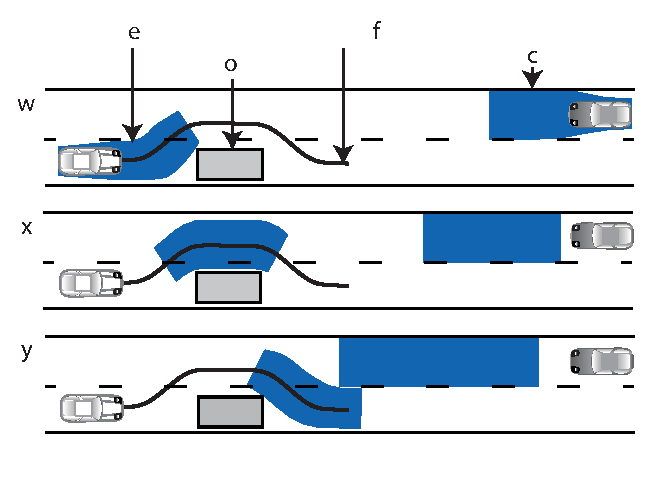
\includegraphics[width=0.8\columnwidth, height=0.74\textheight, keepaspectratio]{./figures/snapshots_blue.eps}
      %\caption{Snapshots of the predicted occupancy of the traffic participant for selected consecutive time intervals.}
\end{frame}


%\begin{frame}{Outline}
%\begin{enumerate}
%\item Item
%\vfill \item Item
%\vfill \item Item
%\vfill \item Item
%\vfill \item Item
%\end{enumerate} 
%\end{frame}



\begin{frame}{SPOT}
SPOT: A tool for set-based prediction of traffic participants $[$2$]$\blfootnote{\tiny $[$2$]$ M. Koschi and M. Althoff, ``SPOT: A tool for set-based prediction of traffic participants,'' in Proc. of the IEEE Intelligent Vehicles Symposium, pp. 1679--1686, 2017.}%\footnote{spot.in.tum.de}
\vspace{1em}

\begin{center}
	{\footnotesize
	\psfrag{a}[r][c]{Obstacle~1}	
	\psfrag{b}[l][c]{Obstacle~2}
	\psfrag{c}[c][c]{Obstacle~3}
	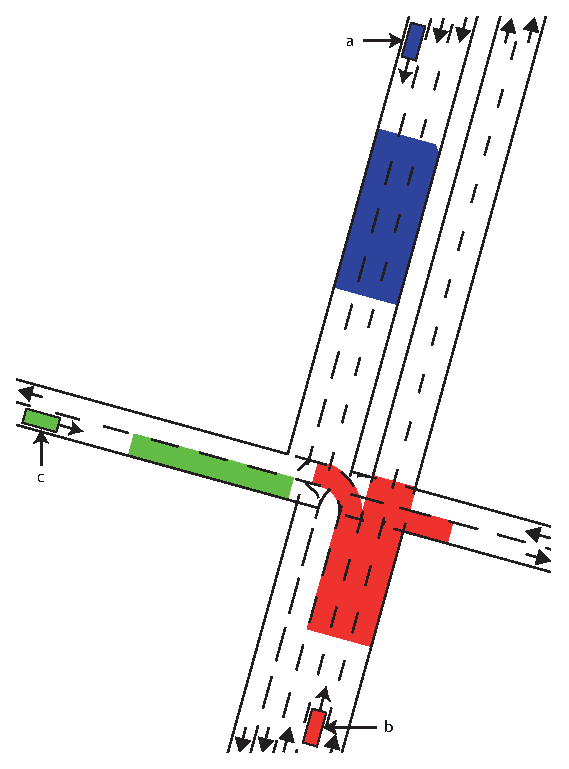
\includegraphics[height=0.5\textheight]{./figures/Scenario_Intersection_Occ_1,5-2,0s_final.eps}
	} \\
	\vspace{1em}
	Initial configuration and $\mathcal{O}(t)$ for $t \in [\unit[1.5]{s}, \unit[2.0]{s}]$
\end{center}

\end{frame}

\begin{frame}{Conclusions}

\begin{itemize}
\item Item
\vfill \item  Item
\vfill \item  Item
\end{itemize}

\end{frame}


begin{frame}
 \frametitle{Ballistic Integration Model }

   Distance and Velocity Equations:
   \begin{columns}[c]
       \begin{column}{0.5\hsize}\centering
       $$ \small s(k+1) = s(k) + dt \cdot v(k) + \frac{dt^2}{2} a(k) $$    
       \end{column}

       \begin{column}{0.5\hsize}
       $$ \small v(k+1) = v(k) + dt \cdot a(k) $$
       \end{column}
   \end{columns}

   \hfil

   \hfil

   \hfil

onslide<2>{

   Acceleration Equations:
   \begin{columns}[c]
       \begin{column}{0.5\hsize}
           \centering
           $$a(k) = \frac{2}{dt^2} \Bigl( s(k+1) - s(k) - dt \cdot v(k) \Bigr)$$
       \end{column}

       \begin{column}{0.5\hsize}
           \centering
           $$ a(k) = \frac{1}{dt} \Bigl( v(k+1) - v(k) \Bigr)$$
       \end{column}
   \end{columns}
}
end{frame}

